In this section, we describe the currently discussed provenance data model. We 
start with a UML class diagram that contains the main important classes 
and then give in the following sections more details for each class and relation.

\subsection{Overview: UML class diagram}
Figure~\ref{fig:classdiagram} shows the UML diagram for an IVOA Provenance Data
Model. It contains the most basic classes; details will be explained in the following sections.
%Its core elements are colored in blue. These core elements can also be found in the W3C Provenance Data
%Model. The pattern defined by these classes is very general and can be reused everywhere where provenance is needed. 

\begin{figure}[h]
\centering
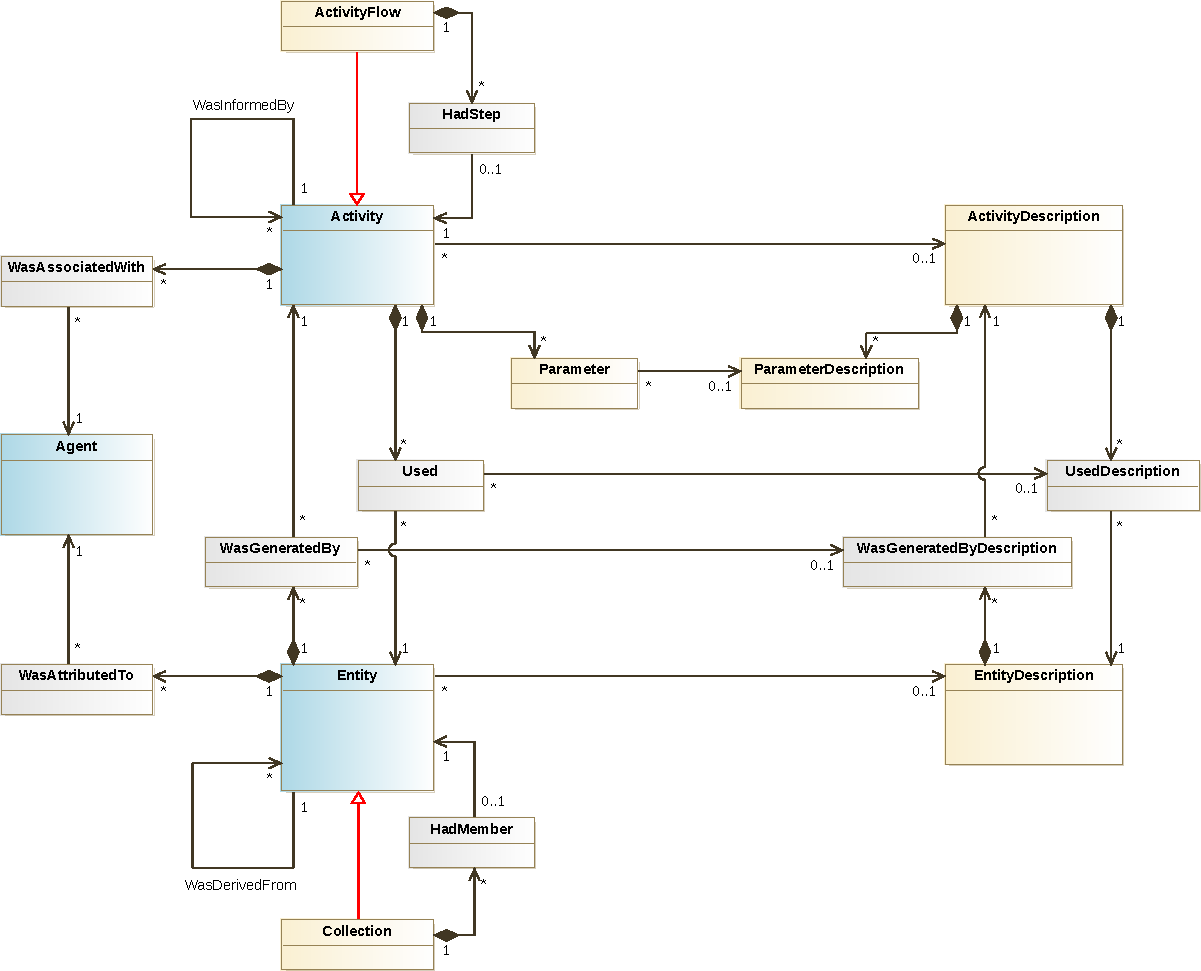
\includegraphics[width=1.0\textwidth]{../datamodel-diagrams/classes-overview.pdf}
\caption{Overview of the classes for the Provenance Data Model in a class diagram. The blue classes are core elements.
%Objects in the blue box also appear in the W3C Provenance Data Model. 
Green classes are links to the IVOA Dataset Data Model.}
\label{fig:classdiagram}
\end{figure}


\subsection{Main classes}\label{sec:core}
% Some examples for different use cases are given in Section \ref{sec:usecases-implementations}.
% The elements of a provenance model can be expressed as a directed graph to capture the causal dependencies. 

\begin{figure}[h]
\centering
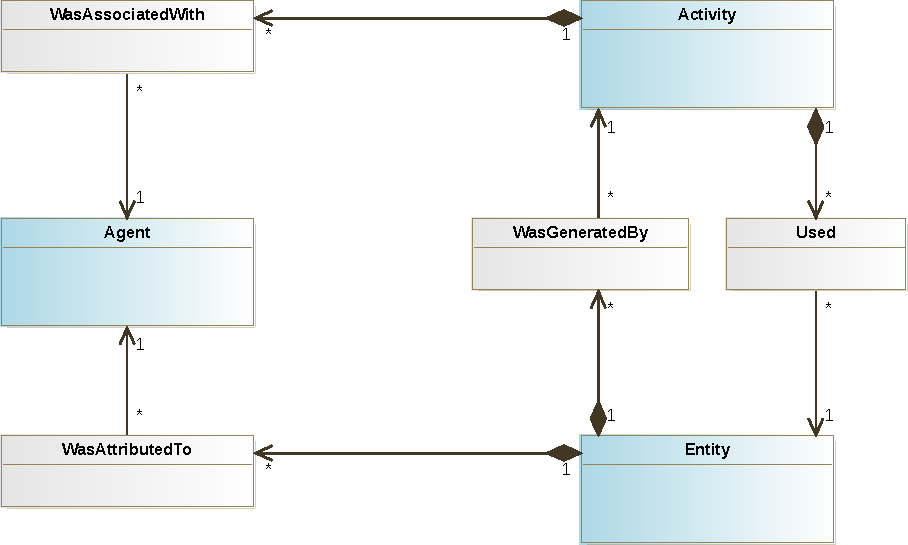
\includegraphics[scale=0.8]{../datamodel-diagrams/classes-core-w3c}
\caption{The main core classes and relations of the Provenance Data Model, which also occur in the W3C model.}
\label{fig:coreclasses}
\end{figure}


The core elements of the provenance data model are \class{Entity}, \class{Activity} and \class{Agent}. 
We chose for these elements the same names as were used in the Provenance Data 
Model of the World Wide Web Consortium (W3C, \cite{std:W3CProvDM}), which defines 
a very abstract pattern that can be reused here. Here are the core classes with 
a short description and some examples:

\begin{itemize}
\item \class{Entity:} a thing at a certain state\\
    examples: data products like images, catalogs, parameter files, calibration data, instrument characteristics

\item \class{Activity:} an action/process or a series of actions, occurs over a period of time, performed on or caused by entities, usually results in new entities\\
    examples: data acquisition like observation, simulation; regridding, fusion, calibration steps, reconstruction

\item \class{Agent:} executes/controls an activity, is responsible for an activity or an entity\\
    examples: telescope astronomer, pipeline operator, principal investigator, software engineer

\end{itemize}

\noindent

We use following relation classes to specify the mapping between the three core 
classes. The names were again chosen to match the W3C model names:
\begin{itemize}
\item \class{WasGeneratedBy:} a new entitiy is generated by an activity\\
        (entity ``image m31.fits'' wasGeneratedBy activity ``observation'')
\item \class{Used:} an entity is used by an activity\\
        (activity ``calibration'' used entities ``calibration data'', ``raw images'')
\item \class{WasAssociatedWith:} agents have responsibility for an activity\\
        (agent ``observer Max Smith'' wasAssociatedWith activity ``observation'')
\item \class{WasAttributedTo:} an entity can be attributed to an agent\\
		(entity ``image m31.fits'' wasAttributedTo ``M31 observation campaign'')
\end{itemize}

Inspired by SimDM (\cite{std:SimDM}), an IVOA  data model for simulation data 
published in May 2012, we also separate descriptions of activities from the 
actual processes and introduce an additional \class{ActivityDescription} class.
\class{Activity} and \class{ActivityDescription} are our Provenance Data Model 
terms for the classes \class{Experiment} and \class{Protocol} in SimDM. 
We also apply the same pattern for \class{Entity} and add an \class{EntityDescription}
class.
Defining such descriptions allows them to be reused, which is very useful 
when performing a series of tasks of the same type, as is typically done in 
astronomy. 

%The W3C-model has the advantage of being already an approved standard, and it 
%contains all the necessary main features needed for a Provenance model for 
%Astronomy. However, it is very general, and by adding reusable prototypes, 
%templates or descriptions for activities and entities,  the model may fit better 
%to the astronomy domain.

It still remains to be seen if this separation into two classes is necessary, 
useful or just nice to have. Currently, we include the descriptions in our model, 
for normalization purposes. But when serialising the provenance one could 
integrate the description side into the other classes, thus producing W3C 
compliant provenance.


\subsubsection{Entity}
Entities in astronomy are usually astronomical or astrophysical datasets in the 
form of images, tables, numbers, etc. But they can also be observation or 
simulation log files or, in a wider sense, also observation proposals, scientific 
articles, or manuals and other documents. An entity is not restricted to being
a file. 
It can even be just a number in a table, depending on how fine-grained the 
provenance shall be described.

Entities in the VO are often called ``dataset'', which could mean a single 
table, an image or a collection of them. The Dataset Data Model 
\citep{std:DatasetDM} specifies an ``IVOA Dataset'' as ``a file or files which 
are considered to be a single deliverable''. If no \class{EntityDescription} is used, then most parts of the \class{Dataset} class can be mapped
directly to the \class{Entity} class, as indicated in Figure \ref{fig:entityclasses}.

The detailed mapping of classes and attributes from the Dataset Data Model 
to \class{Entity} and \class{EntityDescription} are given in Section \ref{sec:dmlinks}. 

\begin{figure}[h]
\centering
\includegraphics[scale=0.5]{../datamodel-diagrams/classes-entity-collection}
\caption{The relation between Entity, Dataset and Collection. The Dataset class belongs to
the IVOA Dataset Data Model.}
\label{fig:entityclasses}
\end{figure}

For entities, we suggest the attributes given in Table 
\ref{tab:entity-attributes}. 
We use the namespace ``prov'', if the attribute also appears in the W3C 
Provenance Data Model.

\begin{table}[h]

\small
\tymax	0.5\textwidth

\textbf{\normalsize Entity}\vspace{0.25em}\\
\begin{tabulary}{1.0\textwidth}{@{}lp{3.5cm}p{2cm}L@{}}
\toprule
\head{Attribute} & \head{W3C ProvDM} & \head{Data type} & \head{Description}\\
\midrule
\textbf{id} & prov:id & (qualified) string & a unique id for this entity (unique in its realm)\\
label        & prov:label & string & a label (to be displayed by clients)\\
type         & prov:type  & string & a provenance type, i.e. one of: prov:collection, prov:bundle, prov:plan, not needed for a simple entity\\
{[description]}  & [prov:description] & string & link to text describing the entity in more detail or link (foreign key) to \class{EntityDescription}\\
access            & -- & string & access rights for the data, values: public, restricted or internal; can be linked to Curation.Rights from ObsCore/DatasetDM\\
\bottomrule
\end{tabulary}
\caption{Attributes of entities. Mandatory attributes are marked in bold.
}\label{tab:entity-attributes}
\end{table}

We discussed further attributes like \emph{size} and \emph{format}, but we decided to treat an
entity of the same content but different format (and thus size) as the same entity,
unless they do not have the same provenance (e.g. when the ``transformation'' activity
for converting one format into another shall be included in the provenance description).

%\TODO{format and size may not be needed, if entities with the same content but different format and size are considered as the same entity.}

The difference between entities that are used as input data or output data 
becomes clear by specifying the relations between the data and activities producing or using these data.
More details on this will follow in Section \ref{sec:entity-activity-relations}.

The types of entities or datasets in astronomy can be predefined using a description
class \class{EntityDescription}.
This class stores entity-related 
attributes, describing the content of the data, which can mainly be derived from 
Dataset Data Model, the general model for observational data.
The description attributes are summarized in Table 
\ref{tab:entitydescription-attributes}.

The \class{EntityDescription} does NOT contain any information about the usage 
of the data, it tells nothing about them being used as input or output. This is 
defined only by the relations (and the relation descriptions) between acitivities
and entities (see Section \ref{sec:entity-activity-relations}).


\begin{table}[h]
\small
\tymax	0.5\textwidth
\textbf{\normalsize EntityDescription}\vspace{0.25em}\\
\begin{tabulary}{\textwidth}{@{}p{2.75cm}p{0cm}p{2cm}L@{}}
\toprule
\head{Attribute} & \head{} & \head{Data type} & \head{Description}\\
\midrule
\textbf{id} & & (qualified) string & a unique identifier for this description\\
label       & & string & a name or label for the entity description\\
description & & string & a decription for this kind of entity\\
docuLink    & & url & link to more documentation\\
dataproduct\_ type  & & string       & from ObsCore data model \citep{std:ObsCore}, if applicable; describes, what kind of product it is (e.g. image, table)\\
dataproduct\_ subtype & & string       & from ObsCore data model, more specific subtype\\
level       & & enum integer & the level of processing or calibration; for ObsCore's calib\_level it is an integer between 0 and 3\\
\bottomrule
\end{tabulary}
\caption{Attributes of \class{EntityDescription}. For simple use cases, 
the description classes may be ignored and its attributes may be used for 
\class{Entity} instead. 
%The utypes may vary depending on the data model, e.g. for simulation data they 
%would point to utypes of SimDM.
}\label{tab:entitydescription-attributes}
\end{table}


\subsubsection{Collection}
Collections are entities that are grouped together and can be treated as one single entity. 
In the provenance sense, they have to have the \emph{same origin}, i.e., they were 
produced by the same activity (which could also be the activity of collecting
data for a publication or similar). The term ``collection'' is 
also used in the Dataset Data Model for grouping datasets.
% (but with a slightly different meaning). 
As an example, a collection 
with the name `RAVE survey' could consist of a number of database tables and spectra files.

%\TODO{Do we allow empty collections? Or should collections always contain at least 1 member? (otherwise they are just prov:entities?)}

The Entity-Collection relation can be modeled using the \emph{Composite} design pattern: 
Collection is a subclass of Entity, but also an aggregation of 1 to many entities, 
which could be collections themselves. 
In order to be compliant to VODML, we model the membership-relation explicitely 
by including a ``HadMember'' class in our model, which is connected to the
``Collection'' class via a composition. It may contain an additional role attribute.

Collections are also known in the W3C model, in the same sense as used here. 
The name for the mapping class, ``HadMember'' was adopted from the W3C model.

An additional class \class{CollectionDescription} is only 
needed if it has different attributes than 
the \class{EntityDescription}. This should therefore only be introduced if a use case requires it.

\paragraph{Advantages of collections:}
\begin{itemize}
\item Collections can be used to collect entities with the same provenance together, 
    in order to hide complexity where necessary. They can be used for defining 
    different levels of detail (granularity).
\item \TODO{Anything else?}
\end{itemize}


\TODO{Find a really strong use case for Collections to convince everyone that they are useful/needed.}



\subsubsection{Activity}
Activities in astronomy include all steps from obtaining data to the reduction of 
images and production of new datasets, like image calibration, bias subtraction, image stacking; 
light curve generation from a number of observations, radial velocity 
determination from spectra, post-processing steps of simulations etc.

The method underlying an activity can be specified by a corresponding 
\class{ActivityDescription} class (previously named \class{Method}, corresponds 
to the \class{Protocol} class in SimDM). This could be, 
for instance, the name of the code used to perform an activity or a more general 
description of the underlying algorithm or process. An activity is then a 
concrete case (instance) of using such a method, with a startTime and endTime, 
and it refers to a corresponding description for further information.

There MUST be exactly zero or  one \class{ActivityDescription} per \class{Activity}. If steps from a 
pipeline shall be grouped together, one needs to create a proper 
\class{ActivityDescription} for describing all the steps at once. This method can then 
be refered to by the pipeline-activity. For grouped activities, also see the 
next section \ref{sec:activity-collection}.

When serializing the data model, the attributes
of the description class may be assigned to the activity in order to produce 
a W3C compliant serialization (same as with Entity/EntityDescription).

\begin{table}[h]

\small
\tymax	0.5\textwidth

\textbf{\normalsize Activity}\vspace{0.25em}\\
\begin{tabulary}{1.0\textwidth}{@{}lp{2.5cm}p{2cm}L@{}}
\toprule
\head{Attribute} & \head{W3C ProvDM} & \head{Data type} & \head{Description}\\
\midrule
\textbf{id} & prov:id  & (qualified) string & a unique id for this activity (unique in its realm)\\
label        & prov:label  & string & a label (to be displayed by clients)\\
\textbf{startTime} & prov:startTime & datetime & start of an activity\\
\textbf{endTime} & prov:endTime  & datetime & end of an activity\\
annotation        & --  & string & additional explanations for the specific activity instance\\
{[description]}  & [prov:description] & string/url/ foreign key & a description for the activity, 
				link to documentation or link to \class{ActivityDescription}\\
\bottomrule
\end{tabulary}
\caption{Attributes of \class{Activity}, their data types and equivalents in the W3C Provenance 
Data Model, if existing. Attributes in bold are \textbf{mandatory}.}
\end{table}


\begin{table}[ht]
\small
\tymax	0.5\textwidth
\textbf{\normalsize ActivityDescription}\vspace{0.25em}\\
\begin{tabulary}{1.0\textwidth}{@{}p{0cm}p{2.5cm}lL@{}}
\toprule
\head{Attribute} & \head{} & \head{Data type} & \head{Description}\\
\midrule
\textbf{id}  & & string & a unique id for this activity description (unique in its realm)\\
label        & & string & a label (to be displayed by clients)\\
type         & & string & type of the activity, from a vocabulary or list, e.g. data acquisition (observation or simulation), reduction, calibration, publication\\
subtype      & & string & more specific subtype of the activity\\
description  & & string & additional free text description for the activity\\
%code         & & string & the code used for this process\\
%version      & & string & a version number for the code\\
docuLink     & & url    & link to further documentation on this process, e.g. a paper, the source code in a version control system etc.\\
\bottomrule
\end{tabulary}
\caption{Attributes of \class{ActivityDescription}.}
\end{table}



\subsubsection{Entity-Activity relations}\label{sec:entity-activity-relations}
\TODO{This section is quite long ... Shorten?}

For each data flow it should be possible to clearly identify entities and 
activities. 
%If the activities shall not be recorded explicitely, one could also 
%use the \emph{Derivation}-relation as suggested in the W3C Provenance Data Model
%to link derived entities to their originals.
Entities are usually results from activities, expressed by a link from 
the entity to its generation activity using the \class{WasGeneratedBy} relation,
and can be used as input for (many) other activities, expressed by the \class{Used} relation.
Thus the information on whether data is used as input or was produced as output of 
some activity is given by the \emph{relation-types} between activities and entities.
%In fact, 
%it would be enough to provide this information just for the relations on the description side (right).
% -- Is this true?

We use two relations, \class{Used} and \class{WasGeneratedBy}, instead of just one
mapping class with a flag for input/output, in order to model the different 
multiplicities explicitely: an entity always has only one (or none) 
\class{WasGeneratedBy} relation, but may be \class{Used} many times as input for 
different activities.


Additionally, input (and also output) data can take different roles in an 
activity. For example, one file could
be a parameter file, another one is the raw image, and the third one is the 
dark field that should be subtracted. Since these roles are very important, 
it must be made explicit which data component needs to fulfill which role as 
input in or output from an activity.
Each activity requires specific roles for each input or output entity, thus 
we store this information on the description side, in the role-attributes for 
the \class{UsedDescription} and \class{WasGeneratedByDescription} relation.

%In W3C, this is partially solved by adding a derivation relation between the Entities (data). Here, we have a mapping-class between Activity and DataEntities as well as between ActivityDescription and DataDescription. The mapping-class at the description side, i.e. between the ActivityDescription and its DataEntityDescriptions, contains additionally a role for each relation, e.g. parameter, dark frame, raw image, etc.  If a dataset is used as input to an activity or if it results from it, will become clear with these roles.


Some example roles are given in Table \ref{tab:entity-roles}.
Note that these roles don't have to be unique, many datasets may play the same role for 
a process. For example, many image entities may be used as science-ready-images for an 
image stacking process.

\begin{table}[h]
\small
\begin{tabulary}{1.0\textwidth}{@{}lL@{}}
\toprule
\head{Name} & \head{Description}\\
\midrule
parameter & \\
dark frame & \\
calibration image & \\
raw image & \\
science-ready image & \\
\bottomrule
\end{tabulary}
\caption{Example values for the entity roles as attributes in the 
\class{UsedDescription} and \class{WasGeneratedByDescription}.}
\label{tab:entity-roles}
\end{table}

The role is in general NOT an attribute for \class{EntityDescription} or \class{Entity}, 
since the same entity (e.g. a specific fits file containing an image) may play 
different roles with different activities. Only if this is not the case, if the 
image can only play the same role everywhere, only then it is an intrinsic 
property of the entity and should be stored in the \class{EntityDescription}.

\TODO{In order to facilitate interoperability, the possible 
entity-roles could be defined and described for each activity by the IVOA community, in a 
vocabulary list or thesaurus.}

\TODO{Roles can be used for checking (validation) if processes use the correct type of entities, 
e.g. check if entity-type matches used-role!}

%Without the mapping tables, the relation between \class{Activity} 
%(\class{ActivityDescription}) and \class{Entity} (\class{EntityDescription})
%would be an aggregation relation, or in other words: an association with the 
%aggregation kind ``shared''. That would be required to ensure that all 
%entities linked to an activity (either as input or output) will survive if 
%the activity is destroyed, since they are almost always shared with other 
%activities. 
%
%By using the mapping tables we make the role of an entity in an activity more 
%explicit and thus can replace the aggregation by a composition relation to the 
%\class{Activity}/\class{ActivityDescription} and simple associations to the 
%individual data components and their descriptions. 


% The derivation relation together with entities is already enough to produce a 
% Data flow view, but in astronomy we are probably even more interested in the 
% Processes (as discussed in our first draft for requirements for provenance).

\TODO{Add an example here! (From discussions in Heidelberg.)}




\subsubsection{Agent}\label{sec:w3c-agent}

An \class{Agent} describes someone who is responsible for a certain task or
entity, e.g. who pressed a button, 
ran a script, performed the observation or published a dataset.
The agent can be a single person, a group of persons (e.g. MUSE WISE Team), a 
project (RAVE) or an institute. 
This is also reflected in the IVOA Dataset Data Model, where \class{Party} 
represents an agent, and it has two subtypes: \class{Individual} and \class{Organization},
which are explained in more detail in Table \ref{tab:agent-types}.
Both types are also used for agent types in the W3C Provenance Data Model, though 
\class{Individual} is called \class{Person} there. 
We do not include the type \class{SoftwareAgent} from W3C, since it is not required for 
our use cases.

\begin{table}[h]
\small
\tymax  0.5\textwidth
\begin{center}
\begin{tabulary}{1.0\textwidth}{@{}lllL@{}}
\multicolumn{3}{c}{\textbf{AgentType}}\\
\toprule
\head{Class} & \head{W3C ProvDM} & \head{DatasetDM} &\head{Comment} \\
\midrule
Agent       & Agent  & Party & \\
Individual  & Person & Individual & a person, specified by name, email, address, 
      (though all these parts may change in time)\\
Organization & Organization & Organization & a publishing house, institute or scientific project\\
\bottomrule
\end{tabulary}
\caption{Types of agents}
\label{tab:agent-types}
\end{center}
\end{table}

A definition of organisations in the sense of the VO is given in the 
IVOA Recommendation on Resource Metadata \citep{std:ResourceMeta}, hereafter 
refered to as RM: ``An organisation is [a] specific type of resource that 
brings people together to pursue participation in VO applications.''
It also specifies further that scientific projects can be considered 
as organisations on a finer level:
``At a high level, an organisation could be a university, observatory, or government
agency. At a finer level, it could be a specific scientific project, space mission,
or individual researcher. A provider is an organisation that makes data and/or services
available to users over the network.''

For each agent a \emph{name} should be specified.
It would also increase the value of the given
information if the (current) affiliation of the agent (and a project leader/group
leader) were specified in order to maximize the chance of finding any contact 
person later on. 
The contact information is needed in case more information about a certain step in the past of a dataset is required,
but also in order
to know who was involved and to fulfill our ``Attribution'' requirement 
(Section~\ref{sec:requirements}), so that proper credits are given to the right 
people/projects.

\begin{figure}[h]
\centering
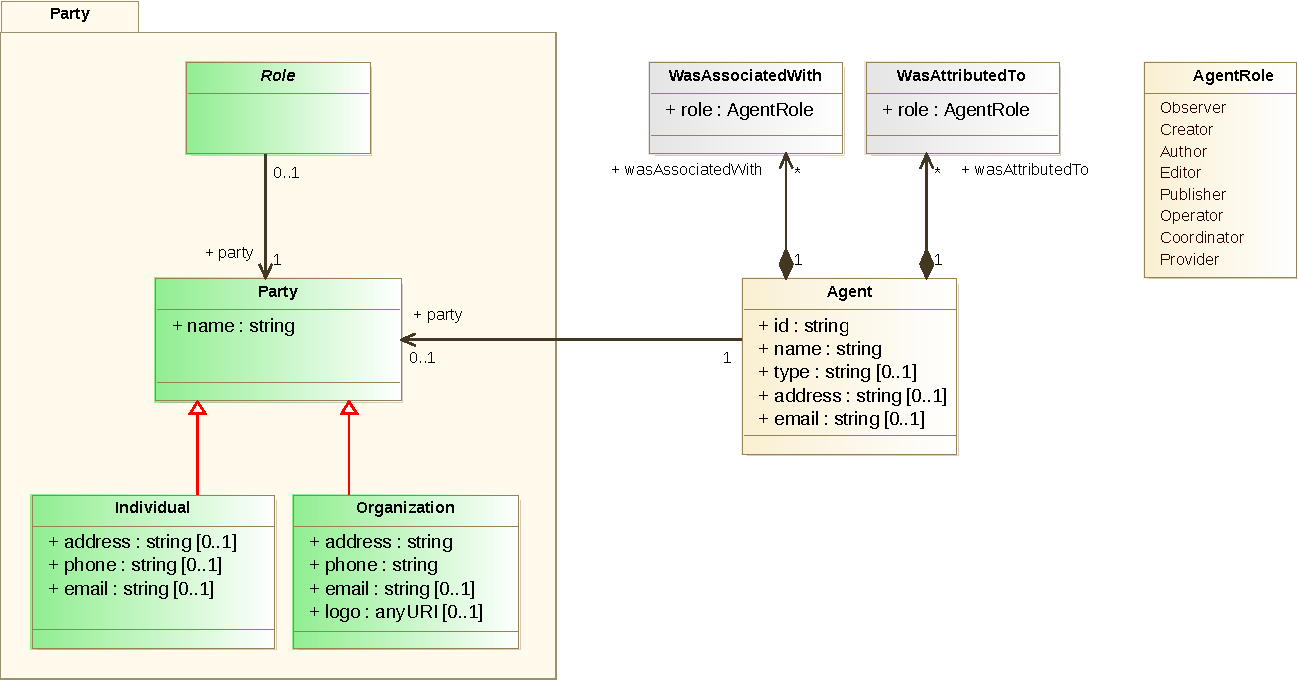
\includegraphics[scale=0.7]{../datamodel-diagrams/agent-relations.pdf}
\caption{The relations between the \class{Agent} class within the Provenance Data Model 
(grey and yellow classes) and with classes from the Dataset Data Model (green).}
\label{fig:agent-relations}
\end{figure}


The relations between \class{Agent} and other classes from the Provenance Data Model and
the IVOA Dataset Data Model are detailed in Figure \ref{fig:agent-relations}.

It is desired to have at least one agent given for each activity (and entity), but it
is not enforced.
% , hence the multiplicity between \class{Entity}/\class{Activity} and the relations
%to the \class{Agent} starts with 0.
There can also be more than one agent for each activity/entity with different \emph{roles} 
and one agent can be responsible for more than one activity or entity. This 
many-to-many relationship is made explicite in our model by adding the two
following relation classes:

\begin{itemize}
\item wasAssociatedWith: relates an \emph{activity} to an agent
\item wasAttributedTo: relates an \emph{entity} to an agent
\end{itemize}

We adopted here the same naming scheme as was used in W3C ProvDM.
Note that the attributed-to-agent for a dataset may be different from the 
agent that is associated with the activity that created an entity. 
Someone who is performing a task is not necessarily given full attribution, 
especially if he acts on behalf of someone else (the project, university, ...).

In order to make it clearer what an agent is useful for, we suggest the
possible roles an agent can have (along with descriptions partially taken from RM)
in Table~\ref{tab:agent-roles}. 
For comparison, SimDM contains following roles 
for their \emph{Contact} class: 
owner, creator, publisher and contributor.


\begin{table}[h]
\small
\tymax	0.5\textwidth
\begin{center}
\begin{tabulary}{1.0\textwidth}{@{}llL@{}}
\multicolumn{3}{c}{\textbf{AgentRoles}}\\
\toprule
\head{prov:role} & \head{prov:type} & \head{Comment} \\
\midrule
author & prov:person & someone who wrote an article, software, proposal\\
contributor & prov:person & someone who contributed to something (but not enough to gain authorship)\\
curator & prov:person & someone who checked and corrected a dataset before publishing\\
editor & prov:person & editor of e.g. an article, before publishing\\
publisher & prov:organization & organization (publishing house, institute) that published something\\
observer & prov:person & observer at the telescope\\
operator & prov:person & performing a given task (executor?)\\
coordinator/PI & prov:person & someone coordinating/leading a project\\
provider & prov:organization & ``an organization that makes data and/or services available to users over the network'' (definition from RM)\\
owner & ?? &  (does anyone own the data?)\\
creator & ?? &  (about the same as author?)\\
\bottomrule
\end{tabulary}
\caption{Roles of agents}
\label{tab:agent-roles}
\end{center}
\end{table}

\TODO{\textbf{Mireille + Francois}: Go through these roles, pick only the necessary ones, crosscheck with other data models.}

This list is \emph{not} complete. We consider providing a vocabulary list for this 
in a future version of this model, collected from (future) implementations of this model.

%\TODO{Do we have a specific use case for fixing the agent-roles? Is anyone 
%going to search for specific roles in the Provenance meta-data?
%Or shall we leave it open, which roles can be defined and just give examples here?}
% ... Yes, just give examples here. Should have a vocabulary list somewhere ...

\begin{table}[h]
\small
\tymax  0.5\textwidth
\begin{center}
\begin{tabulary}{1.0\textwidth}{@{}llp{2cm}L@{}}
\multicolumn{4}{c}{\textbf{Agent}}\\
\toprule
\head{Attribute} & \head{W3C ProvDM} & \head{Data type} & \head{Description}\\
\midrule
id & prov:id & (qualified) string & unique identifier for an agent\\
name & prov:name & string & a common name for this agent; e.g. first name and last name; project name, ...\\
type & prov:type & string & type of the agent: either person or organization\\
\bottomrule
\end{tabulary}
\caption{Agent attributes}
\label{tab:agent-attributes}
\end{center}
\end{table}


%% Additional classes for grouping and short-cuts

\subsubsection{ActivityFlow}\label{sec:activity-collection}
For facilitating grouping of activities (and their related entities etc.)
we introduce the class \class{ActivityFlow}.
It can be used for hiding a part of the workflow or provenance 
description, if different levels of granularity are needed. Figure \ref{fig:provgraph-activityflow}
illustrates an example provenance graph in a detailed level (left side) 
and using the ActivityFlow (right side).


\begin{figure}[h]
\centering
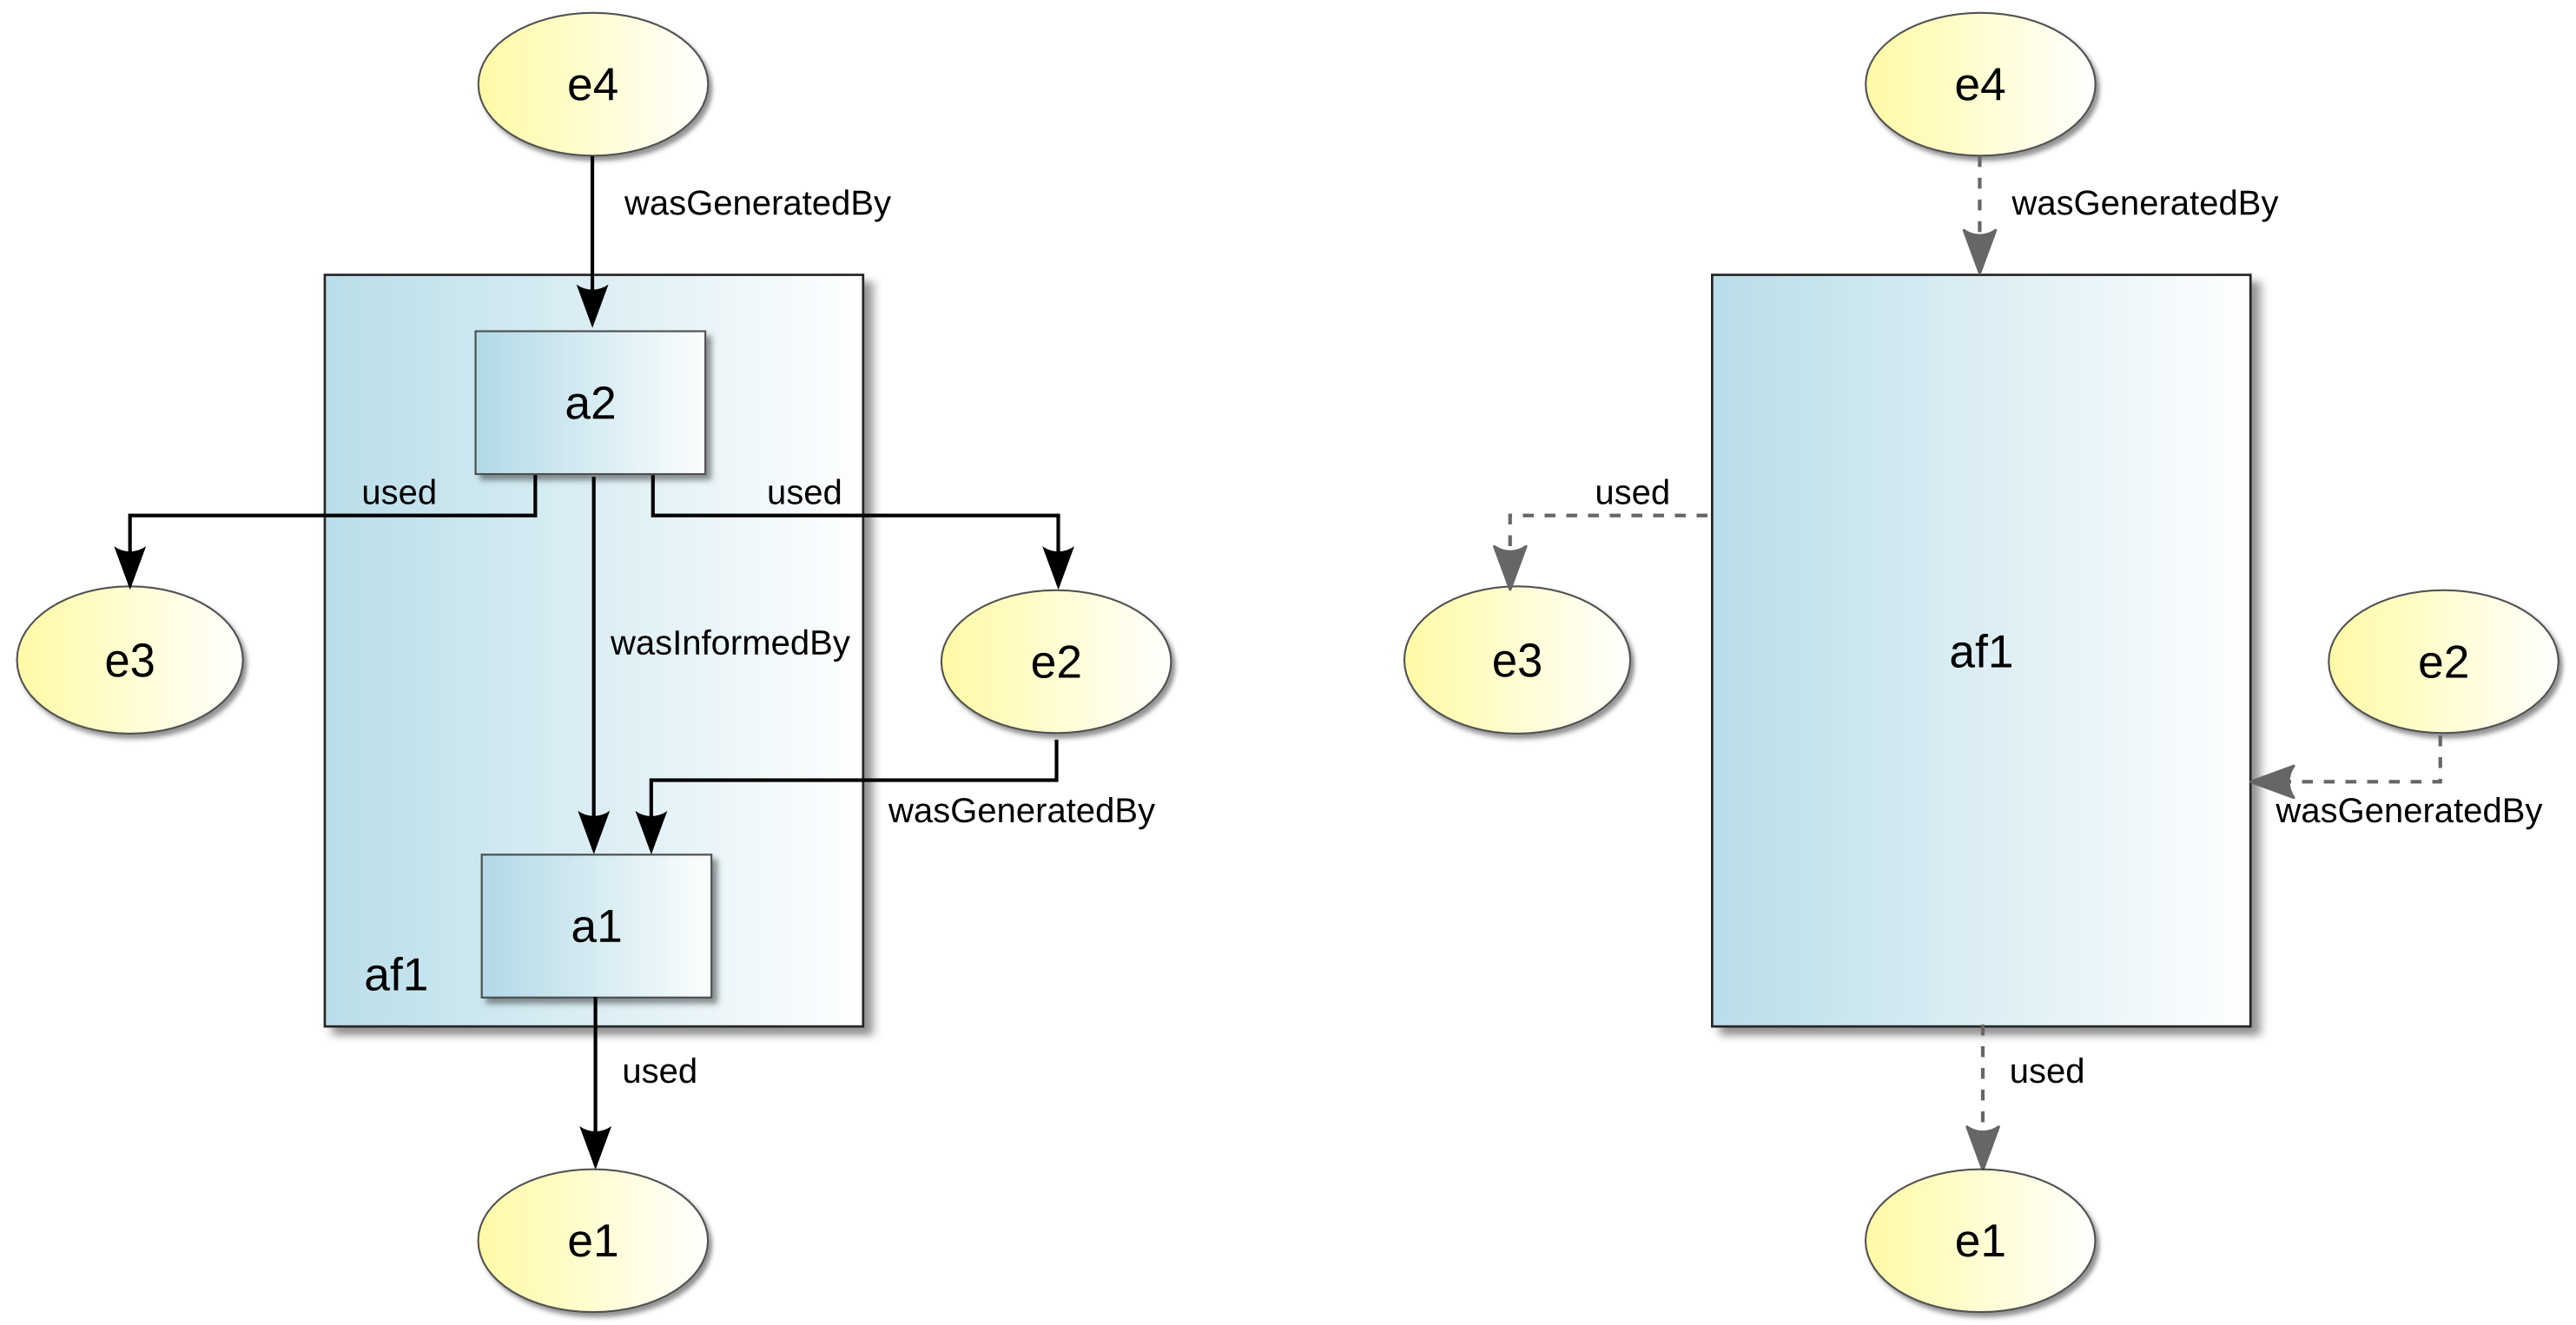
\includegraphics[width=1\textwidth]{../datamodel-diagrams/provgraph-activityflow}
\caption{An example provenance graph. The detailed version is shown on the left side. It also uses 
the shortcut \class{WasInformedBy} to connect two activities where the intermediate entity is not
that interesting.
An ActivityFlow can be used to ``hide'' a part of the provenance graph as is shown on the right side.
Activities are marked by blue rectangles, Entities by yellow ellipses.}
\label{fig:provgraph-activityflow}
\end{figure}

\TODO{BEWARE: Allowing this means that there can be 2 or more wasGeneratedBy-relations
per entity!! This is currently NOT allowed in our model (multiplicity 0..1)! Or shall we 
allow the encapsulating parts of a provenance graph 
only in the view, i.e. on the implementation side?}


In the W3C provenance model, the entity type \class{Plan} is used for workflows and 
provenance descriptions are called \class{Bundle}. However, we do not reuse these 
terms here, since we want to use the class \class{ActivityFlow} as a kind of \class{Activity}
with all the relations and properties that an \class{Activity} also has. 



%while still making it obvious that this 
%group contains activities, we introduce the class \class{ActivityFlow}.
%This can be used for describing workflows or pipelines, or for 
%
%We also allow ActivityCollections to consist of a whole provenance graph of 
%activities and entities being linked together.

\subsubsection{Shortcuts: WasDerivedFrom and WasInformedBy}\label{sec:shortcuts}
The classes \class{WasDerivedFrom} and \class{WasInformedBy} can be used as ``shortcuts'' and 
are used in the same way as the corresponding W3C classes.

\class{WasDerivedFrom} defines the relation that links two entities together, if one entity was derived
from the other entity. In principle, one can find this information also by tracing the 
history of an entity backwards to the generating activity and its input entities. 
The descriptions for activity, entity and their relations should provide enough
information to find the progenitor entity from which an entity was derived.
Nevertheless, we include \class{WasDerivedFrom} for those cases where an explicite 
link between an entity and its progenitor is useful (e.g. for speeding up searches for 
progenitors or if the activity in between is not important).

The class \class{WasInformedBy} links two activities together without defining the
intermediate entities that may have been exchanged. This is useful for e.g. pipelines, 
if the intermediate entities don't play a major role or only exist temporarily, so that
their provenance information is not deemed to be important enough to be recorded.
%``WasInformedBy'' relation (also called ``Communication'' relation, borrowed from W3C's model) 
